\documentclass[gray]{beamer}
\usepackage{graphicx}
\usepackage{tikz}
\usepackage{mathtools}
\usepackage{amssymb}
\usepackage{cite}
% -- To use color white throughout the document
\usepackage{xcolor}
% - To include Greenely logo
\usepackage{textpos}
% - Algorithms --
\usepackage{algpseudocode}% http://ctan.org/pkg/algorithmicx
\usepackage[titlenumbered,ruled]{algorithm2e}
\usepackage{algcompatible}
%
% - Python code --
\usepackage{listings}
%  ----
\usetikzlibrary{positioning}
\usepackage[swedish,english]{babel}
\title[Energy Disaggregation at Greenely] % (optional, only for long titles)
{Energy Disaggregation at Greenely}
\mode<presentation>{}
\author[Eric Leijonmarck]{
\includegraphics[height=2cm,width=2cm]{./figures/greenelylogo.jpg}\\Eric Leijonmarck} % (optional, for multiple authors)

\institute[Royal Institute of Technology - Stockholm]
{
  \inst{}%{1}%
  Royal Insitute of Technology\\
}
\date % (optional)

\begin{document}
\lstset{language=Python}          % Set your language (you can change the language for each code-block optionally)

%   ---   To make the group totally black ---
\bgroup
\newcommand{\norm}[1]{\left\lVert#1\right\rVert}

\setbeamercolor{itemize/enumerate body}{fg=white}
\setbeamertemplate{navigation symbols}{}
\color{white}

%\setbeamercolor{abstract,abstract title,alerted text,author,author in head/foot,author in sidebar,background,background canvas,bibliography entry author,bibliography entry location,bibliography entry note,bibliography entry title,bibliography item,block body,block body alerted,block body example,block title,block title alerted,block title example,button,button border,caption,caption name,date,date in head/foot,date in sidebar,description item,enumerate item,enumerate subitem,enumerate subsubitem,example text,fine separation line,footline,framesubtitle,frametitle,frametitle right,headline,institute,institute in head/foot,institute in sidebar,item,item projected,itemize item,itemize subitem,itemize subsubitem,itemize/enumerate body,itemize/enumerate subbody,itemize/enumerate subsubbody,local structure,logo,lower separation line foot,lower separation line head,math text,math text displayed,math text inlined,middle separation line foot,middle separation line head,mini frame,navigation symbols,navigation symbols dimmed,normal text,normal text in math text,normal text in math text,page number in head/foot,palette primary,palette quaternary,palette secondary,palette sidebar primary,palette sidebar quaternary,palette sidebar secondary,palette sidebar tertiary,palette tertiary,part name,part title,qed symbol,quotation,quote,section in head/foot,section in sidebar,section in sidebar shaded,section in toc,section in toc shaded,section name,section number projected,section title,separation line,sidebar,sidebar left,sidebar right,structure,subitem,,subitem projected,subsection in head/foot,subsection in sidebar,subsection in sidebar shaded,subsection in toc,subsection in toc shaded,subsection name,subsection number projected,subsection title,subsubitem,subsubitem projected,subsubsection in head/foot,subsubsection in sidebar,subsubsection in sidebar shaded,subsubsection in toc,subsubsection in toc shaded,subsubsection number projected,subtitle,title,title in head/foot,title in sidebar,titlegraphic,titlelike,upper separation line foot,upper separation line head,verse}{fg=white}

% --- Set color of presentation to white ----
\setbeamercolor{background canvas}{bg=black}
\setbeamercolor*{frametitle}{fg=white,bg=black}
\setbeamercolor{date in head/foot}{fg=white}
\setbeamercolor{section in head/foot}{fg=white}
\setbeamercolor{section in toc}{fg=black,bg=white}
\setbeamercolor{alerted text}{fg=white}
\setbeamercolor{section in toc}{fg=white}
\setbeamercolor*{structure}{fg=white}
\setbeamercolor*{title}{fg=white}
\setbeamercolor*{author}{fg=white}
\setbeamercolor*{institute}{fg=white}
\setbeamercolor*{date}{fg=white}
\setbeamercolor*{itemize}{bg=white,fg=white}

%\AtBeginSection[]
%{
%  \begin{frame}[plain]
%    \frametitle{Table of Contents}
%    \tableofcontents[currentsection]
%  \end{frame}
%}


% - add the logo of Greenely to each of the pages
\addtobeamertemplate{frametitle}{}{%
\begin{textblock*}{200mm}(.85\textwidth,-1cm)

\includegraphics[height=2cm,width=2cm]{./figures/greenelylogo.jpg}
\end{textblock*}}


% Presentation
% Show a well disposed report, with clear accounts of the project and the results, clear analysis, and well founded argumentation, as well as good language usage, format and scientific accuracy. Show a good ability to orally present with clear argumentation and analysis, and also a good ability to discuss the work.
%%%%%%%%%%%%%%%%%%%%%%%%%%%%%%%
\frame{\titlepage}
%{Greenely}
%{Energy disaggregation, informatics task related to energy efficiency}
%{Discriminative, conditional models}
%{Sparse Coding, Neural Networks}
%{Appliance-level data could reduce consumption by 12\%}
%\{"Smart Meters", collect whole-home level per hour}
%%%%%%%%%%%%%%%%%%%%%%%%%%%%%%
\section{Introduction}
%%%%%%%%%%%%%
\begin{frame}
	\frametitle{Content}
	\framesubtitle{Contents of this presentation}
	\begin{itemize}
		\item{Disaggregation; state of 2015}
		\item{Sparse-coding implementation}
		\item{Results and Extensions}
		\item{Pre-processing data}
		\item{Suggestions on how to proceed next}
	\end{itemize}
\end{frame}
%%%%%%%%%%%%%%%%%%%%%%%%
\begin{frame}
	\frametitle{State of 2015}
	\framesubtitle{Competitors}
	\begin{itemize}
		\item{Smart-meter disaggregation}
		\begin{enumerate}
			\item{\href{http://www.energyefficiency.me/}{EEme, energy disaggregation}}
			\item{\href{http://sensehome.com/}{SenseHome, startup in Boston}}
			\item{Bidgely, PlotWatt, ComEd, Neurio, Navetas, Belkin, Intel}
		\end{enumerate}
		\item{ Hardware Competitors}
		\begin{enumerate}
			\item{\href{http://watty.io/}{Watty, KTH-based start-up}}
			\item{\href{http://www.smappee.com/be_en/}{Smappee, real-time Disaggregation startup}}
		\end{enumerate}
		\item{Overall energy product companies}
		\begin{enumerate}
			\item{\href{http://www.itgfirm.com/}{ITG, signal-processsing company in New York}}
			\item{\href{http://www.britishgas.co.uk/}{British Gas, holistic energy provider}}
			\item{\href{http://www.opower.com/solutions/energy-efficiency}{Opower, energy efficiency}}
		\end{enumerate}
	\end{itemize}
\end{frame}
%%%%%%%%%%%%%%%%%
\begin{frame}
	\frametitle{State of 2015}
	\framesubtitle{Research}
	\begin{itemize}
		\item{Research in Energy Disaggregation}
			\begin{figure}[!ht]
				\colorbox{white}{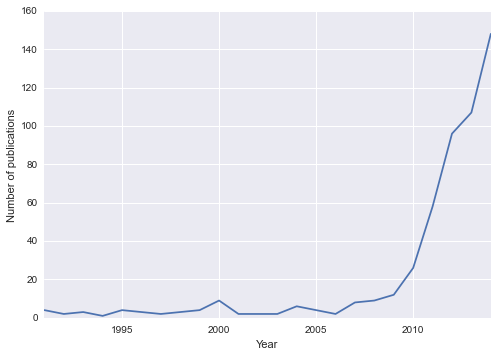
\includegraphics[scale=0.50]{./figures/growth}}
			\end{figure}
			\centering
			Increase at 2010 from 20 - 140 in 4 years
	\end{itemize}
\end{frame}
%%%%%%%%%%%%%%%%
%%%%%%%%%%%%%%%%%
\begin{frame}
	\frametitle{State of 2015}
	\framesubtitle{Challenge}
	\begin{itemize}
		\item{Challenge}
		\begin{figure}[!ht]
			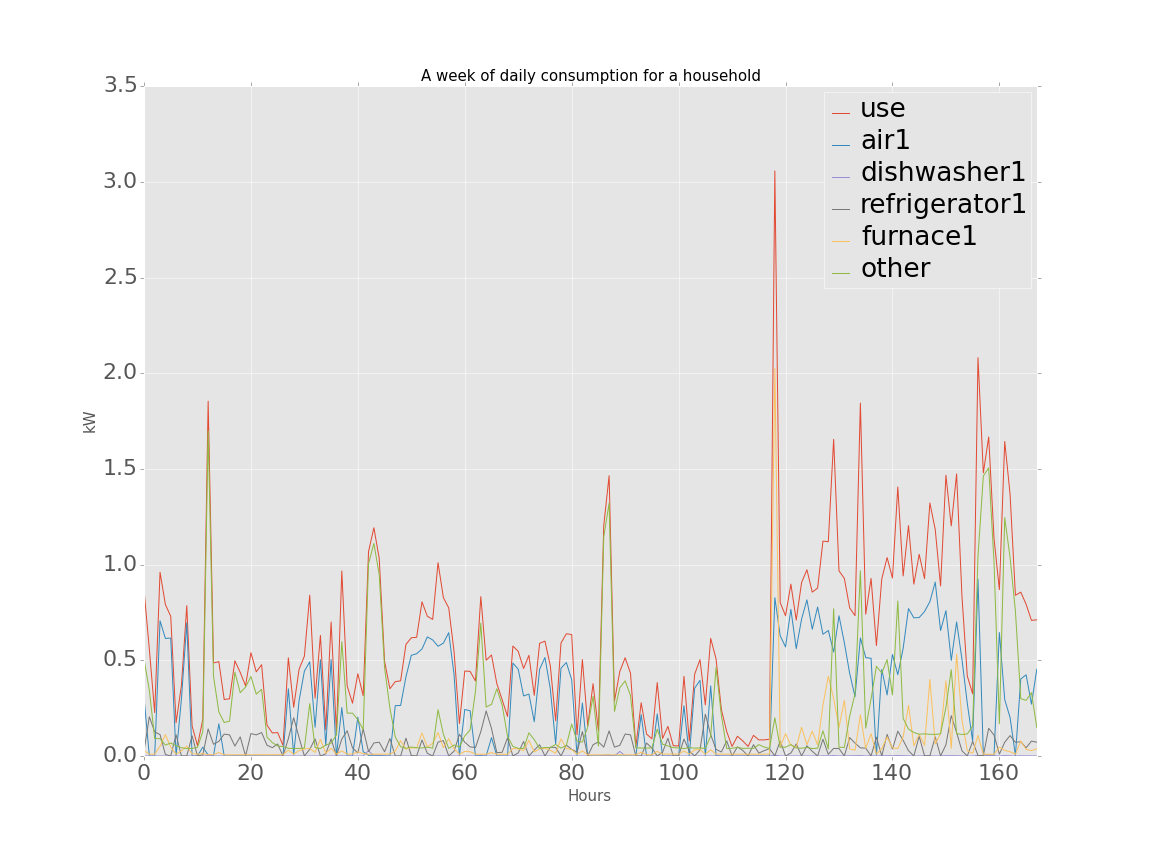
\includegraphics[scale=0.18]{./figures/weekconsump}
		\end{figure}
	\end{itemize}
	\begin{itemize}
		\item{Lots of methods one common denominator, Data}
		\item{Perform unsupervised on test, and supervised on scaled houses}
	\end{itemize}
\end{frame}
%%%%%%%%%%%%%%%%
%%%%%%%%%%%%%%%%%
\begin{frame}
	\frametitle{State of 2015}
	\framesubtitle{Solution}
	\begin{itemize}
		\item{Data, Data-preparation, Data-data, Data-data-data}
	\end{itemize}
	\begin{itemize}
		\item{Ed Freeman, More Data or Better Algorithms?}
		\begin{enumerate}
			\item{Having a good problem to work on}
			\item{Having a good approach to that problem}
			\item{Having decent data. Quality is much more important than quantity}
			\item{Handling the data well -- good transforms, good missing value handling, making sure that all approaches make sense for the problem.}
		\end{enumerate}
	\end{itemize}
\end{frame}
%%%%%%%%%%%%%%%%
%%%%%%%%%%%%%%%%%%%%%%%%%%%%%%
\section{Input}
\begin{frame}
\frametitle{Input data}
\framesubtitle{We have $1:k$ appliances}
\begin{itemize}
\item{We define one class (e.g. heater) $\mathbf{X}_i \leftarrow 1,\dots, k$}
\item{Where $\mathbf{X}_i \in \mathbb{R}^{T \times m}$, $T$ hourly week data for $m$ houses}
\item{\textbf{One} aggregated household $\bar{\mathbf{X}} \leftarrow \sum_{i:k} \mathbf{X}_i$}
\item{Assuming we have individual energy readings $\mathbf{X}_1,\dots,\mathbf{X}_k$}
\item{Goal: test with new data $\bar{\mathbf{X}}'$ to components $\mathbf{X}_1',\dots,\mathbf{X}_k'$}
\end{itemize}
\end{frame}
%%%%%%%%%%%%%%%%%%%%%%%%%%%%%%
\section{Input}
\begin{frame}
\frametitle{Input data}
\framesubtitle{We have $1:k$ appliances}
\centering
\begin{equation*}
\underbrace{\mathbf{X}_i \in \mathbb{R}^{T \times m}}
\end{equation*}

\begin{equation*}
\begin{bmatrix}
\text{App} & \mathbf{x}_1^{(j)} & \cdots & & \mathbf{x}_1^{(m)}\\
1h & 0.8 kWh & \cdot & & \cdot \\
2h & 0.7 kWh & \cdot & & \cdot \\
\vdots & \vdots & \cdot & & \cdot \\
168h & 0.1kWh & \cdot & &  \cdot
\end{bmatrix}
\end{equation*}
\textit{How do we get this format?}
\end{frame}
%%%%%%%%%%%%%%%%%%%%%%%%%%%%%
\section{Pre-processing}
\begin{frame}
	\frametitle{Pre-processing raw-data}
	\begin{itemize}
		\item{Number of missing values in data}
		\item{When missing - what to do?}
		\item{These points need to be considered before dealing with any algorithm}
		\item{Demonstation of processing}
	\end{itemize}
\end{frame}
% - Nested pretraining using the components of the trained training samples
%%%%%%%%%%%%%%%%%%%%%%%%%%%%%%%%%%%%%%%%%%%%%%%%
\section{Sparse coding pre-training}
\begin{frame}
\frametitle{Sparse coding pre-training}
\framesubtitle{pre-train activations and basis vectors}
\begin{algorithm}[H]
\caption{Dicriminative disaggregation sparse coding}
\label{alg:DDSC}
\SetKwInOut{Input}{input}
\Input{data points for each individual source $\mathbf{X}_i \in
\mathbb{R}^{T \times m}, i = 1:k,$ regularization $\lambda
\in \mathbb{R}_+$, with gradient step size $\alpha \in \mathbb{R}_+$.}
\begin{algorithmic}[1]
\Statex{  \textbf{Sparse coding pre-training:}}
\Statex{  \hspace{0.2in} 1. Initalize \textbf{B}$_i$, $\mathbf{A}_i ; \geq 0$, scale columns $\mathbf{B}_i$ s.t. $\norm{ \mathbf{b}_i^{(j)}}_2 =1$}
\Statex{ \hspace{0.2in} 2. For each $i=1,\dots,k,$ iterate until convergence: }
\Statex \hspace{0.4in} $\mathbf{A_i} \leftarrow \arg \! \min_{A \geq 0} \norm{\mathbf{X}_i - \mathbf{B}_i\mathbf{A}}_F^2 + \lambda \sum_{p,q} \mathbf{A}_{pq}$
\Statex \hspace{0.4in} $\mathbf{B}_i \leftarrow  \arg \! \min_{B \geq 0,\norm{\mathbf{b}^{(j)}}_2 \leq 1} \norm{\mathbf{X}_i - \mathbf{B} \mathbf{A}_i }_F^2$
\end{algorithmic}
\end{algorithm}
\end{frame}
% - Nested pretraining using the components of the trained training samples
%%%%%%%%%%%%%%%%%%%%%%%%%%%%%%%%%%%%%%%%%%%%%%%%
\section{DDT}
\begin{frame}
\frametitle{Discriminiative disaggregation training}
\framesubtitle{perceptron algorithm}
\begin{algorithm}[H]
\caption{Dicriminative disaggregation sparse coding}
\label{alg:DDSC}
\begin{algorithmic}[1]
\Statex \textbf{Discriminative disaggregation training:}
\Statex  \hspace{0.2in} 3. Set $\mathbf{A}_{1:k}^* \leftarrow \mathbf{A}_{1:k},\hat{\mathbf{B}}_{1:k} \leftarrow \mathbf{B}_{1:k}.$
\Statex  \hspace{0.2in} 4. Iterate until convergence:
\Statex \hspace{0.4in} $\hat{\mathbf{A_{1:k}}} \leftarrow \arg \! \min_{A_{1:k} \geq 0} F\left( \bar{\mathbf{X}},\tilde{\mathbf{B}}_{1:k},\mathbf{A}_{1:k} \right)$
\Statex \hspace{0.4in} $\tilde{\mathbf{B}} \leftarrow \left[ \tilde{\mathbf{B}} - \alpha \left( (\bar{\mathbf{X}} - \tilde{\mathbf{B}}\hat{\mathbf{A}})\hat{\mathbf{A}}^T - (\bar{\mathbf{X}}-\tilde{\mathbf{B}}\mathbf{A}^*)(\mathbf{A}^*)^T \right) \right]_+$
\Statex \hspace{0.4in} $\forall \quad i,j,\mathbf{b}_i^{(j)} \leftarrow \mathbf{b}_i^{(j)} / \norm{\mathbf{b}_i^{(j)}}_2$
\Statex \textbf{Given aggregated test examples $\bar{\mathbf{X}}'$}
\Statex \hspace{0.2in} 5. $\hat{\mathbf{A}}'_{1:k} \leftarrow \arg \! \min_{\mathbf{A}_{1:k} \geq 0} F(\bar{\mathbf{X}}',\tilde{\mathbf{B}}_{1:k},\mathbf{A}_{1:k})$
\Statex \hspace{0.2in} 6. Predict $\hat{\mathbf{X}}_i' = \mathbf{B}_i\hat{\mathbf{A}}_i'$
\end{algorithmic}
\end{algorithm}
\note{Learning Structured Prediction Models: A Large Margin Approach}
\end{frame}

% - set basis and actibation as trained from pre-training
% - gradiant step-size
% - perceptron algorithm, updating tilde-B
% - Learning Structured Prediction Models: A Large Margin Approach

% - F : stands for the Frobeus norm

%%%%%%%%%%%%%%%%%%%%%%%%%%%%%%%%%%%%%%%%%%%%%%%%
% - total energy priors, we evaluate the norm (total energy) also
% - we lasso in the atoms and take out what is valuable by L2


%%%%%%%%%%%%%%%%%%%%%%%%%%%%%%%%%%%%%%%%%%%%%%%
\section{DDT}
\begin{frame}
\frametitle{Trained models}
\framesubtitle{DDSC}
\begin{figure}[H]
\centering
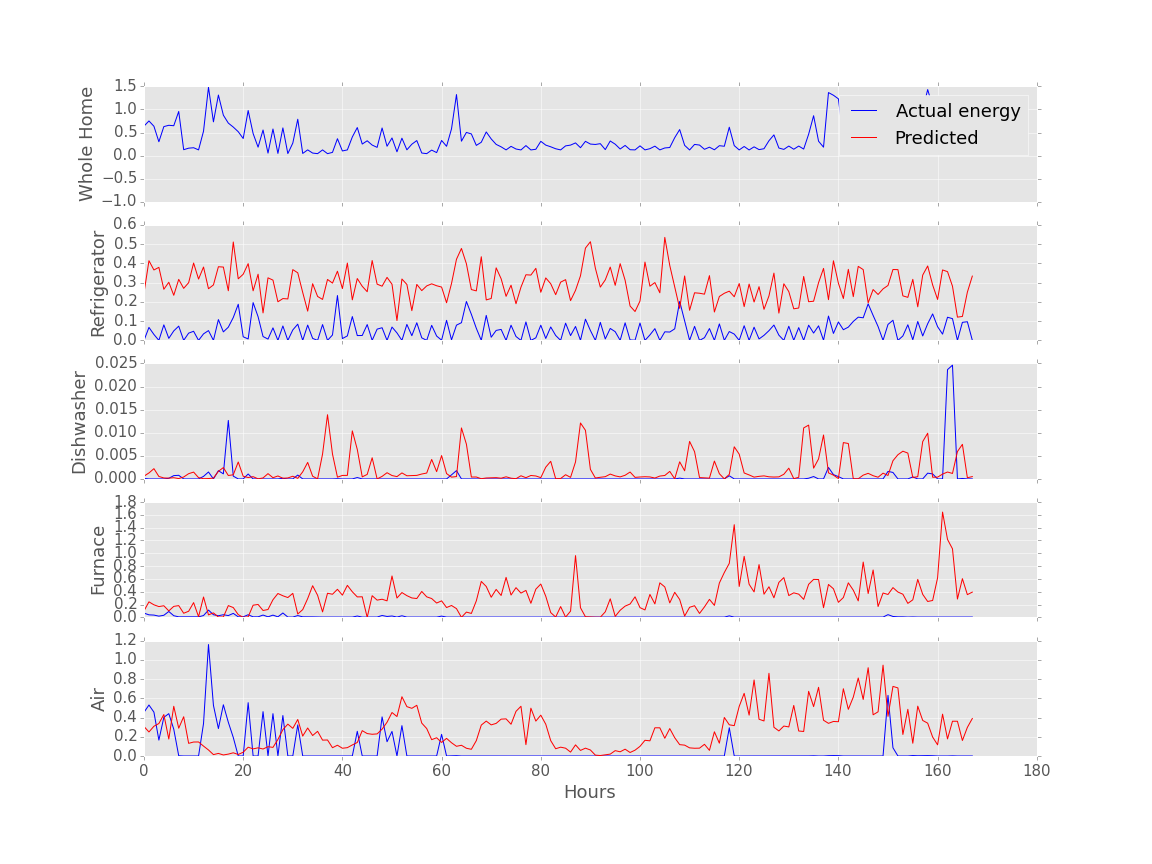
\includegraphics[scale=0.20]{./figures/appliances.png}
%\caption{Example predicted energy profiles and total energy percentages (best viewed in color). Blue lines show the true energy usage, and red the predicted usage, both in units of kWh.}
\end{figure}
\centering
Finds patterns within the data
\end{frame}
%%%%%%%%%%%%%%%%%%%%%%%%%%%%%%%%%%%%%%%%%%%%%%%
\section{DDT}
\begin{frame}
\frametitle{Tests}
\framesubtitle{DDSC}
\begin{equation*}
\text{Accuracy of Week} \equiv \frac{\sum_{i,q} \min \left\{ \sum_p ( \mathbf{X}_i)_{pq}, \sum_p ( \mathbf{B}_i,\hat{\mathbf{A}_i)_{pq}} \right\}}{\sum_{p,q} \bar{\mathbf{X}}_i_{p,q}}
\end{equation*}
\centering
The overlap of the predicted appliance use and the actual appliance usage.
\end{frame}
% - instead of using average, they use total-week accuracy of the prediction system.
%%%%%%%%%%%%%%%%%%%%%%%%%%%%%%%%%%%%%%%%%%%%%%%
\section{DDT}
\begin{frame}
	\frametitle{Tests}
	\framesubtitle{DDSC}
	\begin{figure}
		\centering
		\includegraphics{name}
	\end{figure}
\end{frame}
%%%%%%%%%%%%%%%%%%%%%%%%%%%%%%%%%%%%%%%%%%%%%%%
\section{Extensions}
\begin{frame}
	\frametitle{Extensions}
	\framesubtitle{DDSC}
	\begin{itemize}
		\item{Gridsearch across hyperparameters}
		\item{Clustering - label data}
		\item{Adding extensions to the model, through Andrew}
	\end{itemize}
	Total energy priors: \\
	\vspace{0.1in}
	$F_{TEP}(\bar{\mathbf{X}},\mathbf{B}_{1:k},\mathbf{A}_{1:k}) = F(\bar{\mathbf{X}},\mathbf{B}_{1:k} \mathbf{A}_{1:k}) + \lambda_{TEP}\sum_{i=1}^k \norm{\mu_i\mathbf{1}^T-\mathbf{1}^T\mathbf{B}_i\mathbf{A}_i}^2_2$ \\
	\vspace{0.1in}
	Group Lasso: \\
	$F_{GL}(\bar{\mathbf{X}},\mathbf{B}_{1:k},\mathbf{A}_{1:k}) = F(\bar{\mathbf{X}},\mathbf{B}_{1:k} \mathbf{A}_{1:k}) + \lambda_{GL}\sum_{i=1}^k \sum_{j=1}^m \norm{\mathbf{a}_i^{(j)}}_2$ \\
\end{frame}
%%%%%%%%%%%%%%%%%%%%%%%%%%%%%%
\section{Suggestions}
\begin{frame}
\frametitle{Suggestions}
\framesubtitle{DDSC}
\begin{itemize}
\item{Data, Data, DATA}
	\begin{figure}
		
\includegraphics[scale=.3]{./figures/mydata}
	\end{figure}
\item{Quality data == better models. Period}
\item{Model using fewest assumptions is most likely to be correct.}
\item{Simple algorithm quality data}
\item{All models are wrong, but some are useful. (George E. P. Box)}
\end{itemize}
\end{frame}

%%%%%%%%%%%%%%%%%%%%%%%%%%%%%%
%%%%%%%%%%%%%%%%%%%%%%%%%%%%%%
\section{Suggestions}
\begin{frame}
	\frametitle{Suggestions}
	\framesubtitle{DDSC}
	\begin{figure}
		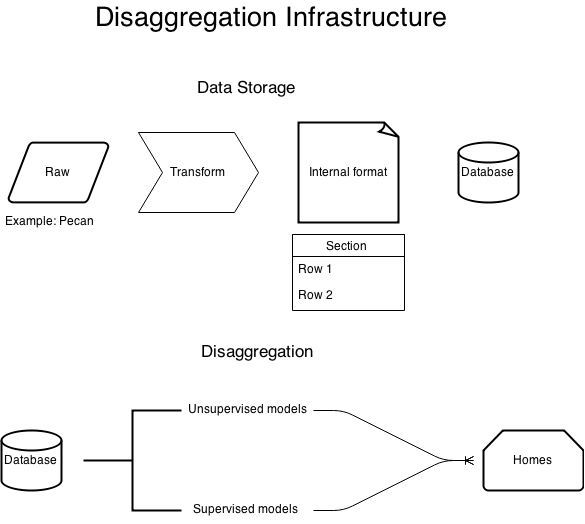
\includegraphics[scale=.36]{./figures/greenelyDisaggregation}
	\end{figure}
\end{frame}
%%%%%%%%%%%%%%%%%%%%%%%%%%%%%%
\begin{frame}
\begin{center}
\huge
Thank you!
\normalsize \\
\vspace{0.3in}
Questions?
\end{center}
\end{frame}

\egroup
\end{document}
